\section{Grafische Benutzeroberfläche}
\label{sec:gui}
Mein Aufgabenschwerpunkt innerhalb unserer Gruppe war die Entwicklung einer bedienbaren graphischen Benutzeroberfläche und die Implementierung wesentlicher Funktionen innerhalb dieser. Deswegen werde ich nachfolgend auf die Funktionalitäten unserer in Abbildung \ref{fig:teaser} zu sehenden GUI sprechen. Eine vollständige Übersicht mit allen HTML Elementen sowie Funktionalitäten dieser findet sich in der Tabelle \ref{tab:gui_funcs}. \\

\subsection{Die Zeichenfläche}
Den meisten Platz unserer Simulation nimmt die Zeichenfläche an sich ein. Diese ist aus insgesamt drei HTML Canvas Elementen aufgebaut: \\

\begin{itemize}
\item Die zwei Seile mit dem eingespannten Stift stellen ein eigenes Canvas im \glqq{}Vordergrund\grqq{} dar.
\item Für das per Radiobutton einblendbare Koordinatensystem mit der Einzeichnung einer grün umrandeten Zeichenfläche habe ich mich auch für ein eigenes Canvas entschieden. 
\item Das Whiteboard, auf dem gezeichnet  wird, stellt ein eigenes Canvas dar. Auf diesem werden Pixel farbig eingezeichnet; Denkbar wäre hier eine Speicherung verschiedener Pixel oder Zustände, um beliebig innerhalb der Simulation vor- und zurückzuspulen zu können (das konnten wir leider aufgrund mangelnder Zeit nicht mehr implementierten; Zu weiterführenden Ideen von uns sei auch hier wieder auf Linos Bericht verwiesen)
\end{itemize}

Diese Entscheidung, drei verschiedene Canvas zu implementieren, brachte unserer Gruppe zwei entscheidende Vorteile: Einerseits war es nun deutlich einfacher, verschiedene Elemente auszublenden, indem wir einfach die jeweiligen Canvas mittels Befehlen wie \glqq{}canvas.clearRect()\grqq{} geleert oder gefüllt haben. Andererseits konnte ich so die Performance unserer Algorithmen deutlich verbessern, da wir davor bei jedem neu gemalten Pixel die bisherigen Pixel gelöscht und alles neu gezeichnet haben. Diese Methode funktionierte auch, allerdings wurde schnell klar, dass das nicht gut mit der Eingabegröße skalieren und wir deutliche Probleme bei komplexeren Bildern mit extremst vielen Pixeln haben würden (In jeder Iteration müsste bei Pixel $n$ alle Pixel $\in \{1,...,n-1\}$ gelöscht werden).


\subsection{Grundlegende Steuerung}
\label{sec:steering}
Rechts von der  eben behandelten Zeichenfläche finden sich verschieden Reiter, dieses Unterkapitel beschäftigt sich mit dem ersten Reiter \glqq{}Simulation\grqq{}. Die anderen Reiter werden in den nachfolgenden Unterkapiteln beschrieben. \\
Zur Steuerung der Simulation operiert unserer Algorithmus auf zwei global angelegten booleschen Variablen $running$ und $pause$. $running$ gibt an, ob die Simulation gerade läuft und $pause$, ob die laufende Simulation angehalten werden soll. Durch Flippen der Variable $pause$ bei Drücken des Buttons \glqq{}Pause/Resume\grqq{} und Abfragen dieser Variablen mittels \glqq{}Busy-Waiting\grqq{} (nicht optimal, reicht aber für unsere Zwecke), war es uns möglich, die Simulation nach Belieben anzuhalten und fortzuführen. \\
Auch kann der aktuelle Wert der Variable $running$ beliebig innerhalb des Algorithmus abgefragt werden und falls dieser wahr ist, der aktuelle  Codeblock beendet werden. Diese Variable wird bei Druck auf den \glqq{}Restart\grqq{}-Button auf den Wert $false$ gesetzt. \\
Der Start-Button erfüllt die Aufgabe einer Initialisierung vor jedem Durchlauf ($running$ auf $true$ und $pause$ auf $false$ setzen, Canvas leeren, usw.) und erscheint ausgegraut, sollte die Simulation gerade laufen (also $running$ wahr sein) oder noch keine Winkelsequenz geladen sein (s. Sektion \ref{sec:paras}). \\
Das Verhalten von $pause$ und $running$ innerhalb eines Simulationsalgorithmus (Näheres zur Implementierung davon bei Lino) ist in dem untenstehenden Pseudocode verdeutlicht:

\begin{algorithm}
\caption{Pause/Resume \& Restart}\label{alg:pause_restart}
\begin{algorithmic}[1]
\Require $pause, resume$
\Ensure $/$
\While{Simulation läuft}
	\State Berechne und zeichne
	\While{$pause$}
		\State \texttt{sleep(100)}  \Comment{Pause für 0.1 Sekunden}
	\EndWhile
	\If{!running}
    	\Return						\Comment{Stoppt Simulation}
	\EndIf
\EndWhile
\end{algorithmic}
\end{algorithm}

Darunter finden sich zwei Funktionen, mit denen man sich ein unter der Zeichnung liegendes Koordinatensystem bzw. die Seile und den Stift anzeigen lassen kann. \\
Startet man die Simulation, so wird im unteren Reiter \glqq{}Logs\grqq{} eine kleine  Übersicht über  die aktuelle Winkelsequenz und einer Fehleranzeige angezeigt. Standardmäßig läuft die Simulation weiter, wenn Fehler gefunden werden (außerhalb des Zeichenbereiches o.Ä.); Mithilfe der letzten Checkbox \glqq{}Stop on errors\grqq{} lässt sich dieses Verhalten ändern. \\
Die Geschwindigkeit, in der das gewünschte Bild gezeichnet wird, ist durch einen Slider darunter einstellbar. Näheres zu meiner Implementierung der Animation erkläre ich in Kapitel \ref{sec:final_anim}.

\subsection{Einstellen gewünschter Parameter}
\label{sec:paras}
Die Elemente des zweiten Reiters \glqq{}Variablen\grqq{} besitzen die Optionen, den Spulendurchmessers des Motors sowie bestimmte Maße zu ändern, um die Simulation flexibler zu gestalten. \\
Standardmäßig habe ich die im Rahmen des Praktikums festgelegten Abmessungen implementiert. Diese sind ein Spulendurchmesser von 16mm und stellen das Whiteboard mit dem darauf befindlichen Zeichenbereich dar und sind der Grafik \ref{fig:abmessungen} zu entnehmen. \\
Durch einen Slider kann der Benutzer den gewünschten Spulendurchmesser von 8mm bis 32mm frei wählen. Für diesen Bereich und eine Schrittgröße von 8mm habe ich mich wegen der in der Praxis benutzten Durchmesser sowie der Übersichtlichkeit entschieden. Die Änderung des Spulendurchmessers lässt sich als Skalierung des gezeichneten Bilds auffassen, da sich pro Schritt die auf- bzw. abgerollte Länge des Seils durch den Umfang der Spule, welche das Seil hält, berechnen lässt. \\
In den sechs weiteren Feldern können nun die gewünschten Maße (in folgender Reihenfolge) eines neuen Whiteboardes, einer neuen Zeichenfläche  und eines neuen Startpunktes definiert werden. Dabei ist zu beachten, dass die Zeichenfläche auf dem Canvas immer zentriert wird und einen Abstand von 4cm vom unteren Rand des Canvas hat. Diese Implementation war ein Wunsch von einer Gruppe und vereinfacht den Prozess, indem nicht nochmal extra Punkte für die Zeichenfläche  eingegeben werden müssen. An dieser Stelle sei zudem dran erinnert, dass der Startpunkt nur den initialen Startpunkt ändert, nicht aber den Punkt, ab wo gezeichnet wird (wie in Kapitel \ref{sec:input} erwähnt).

\begin{figure}[ht]\centering
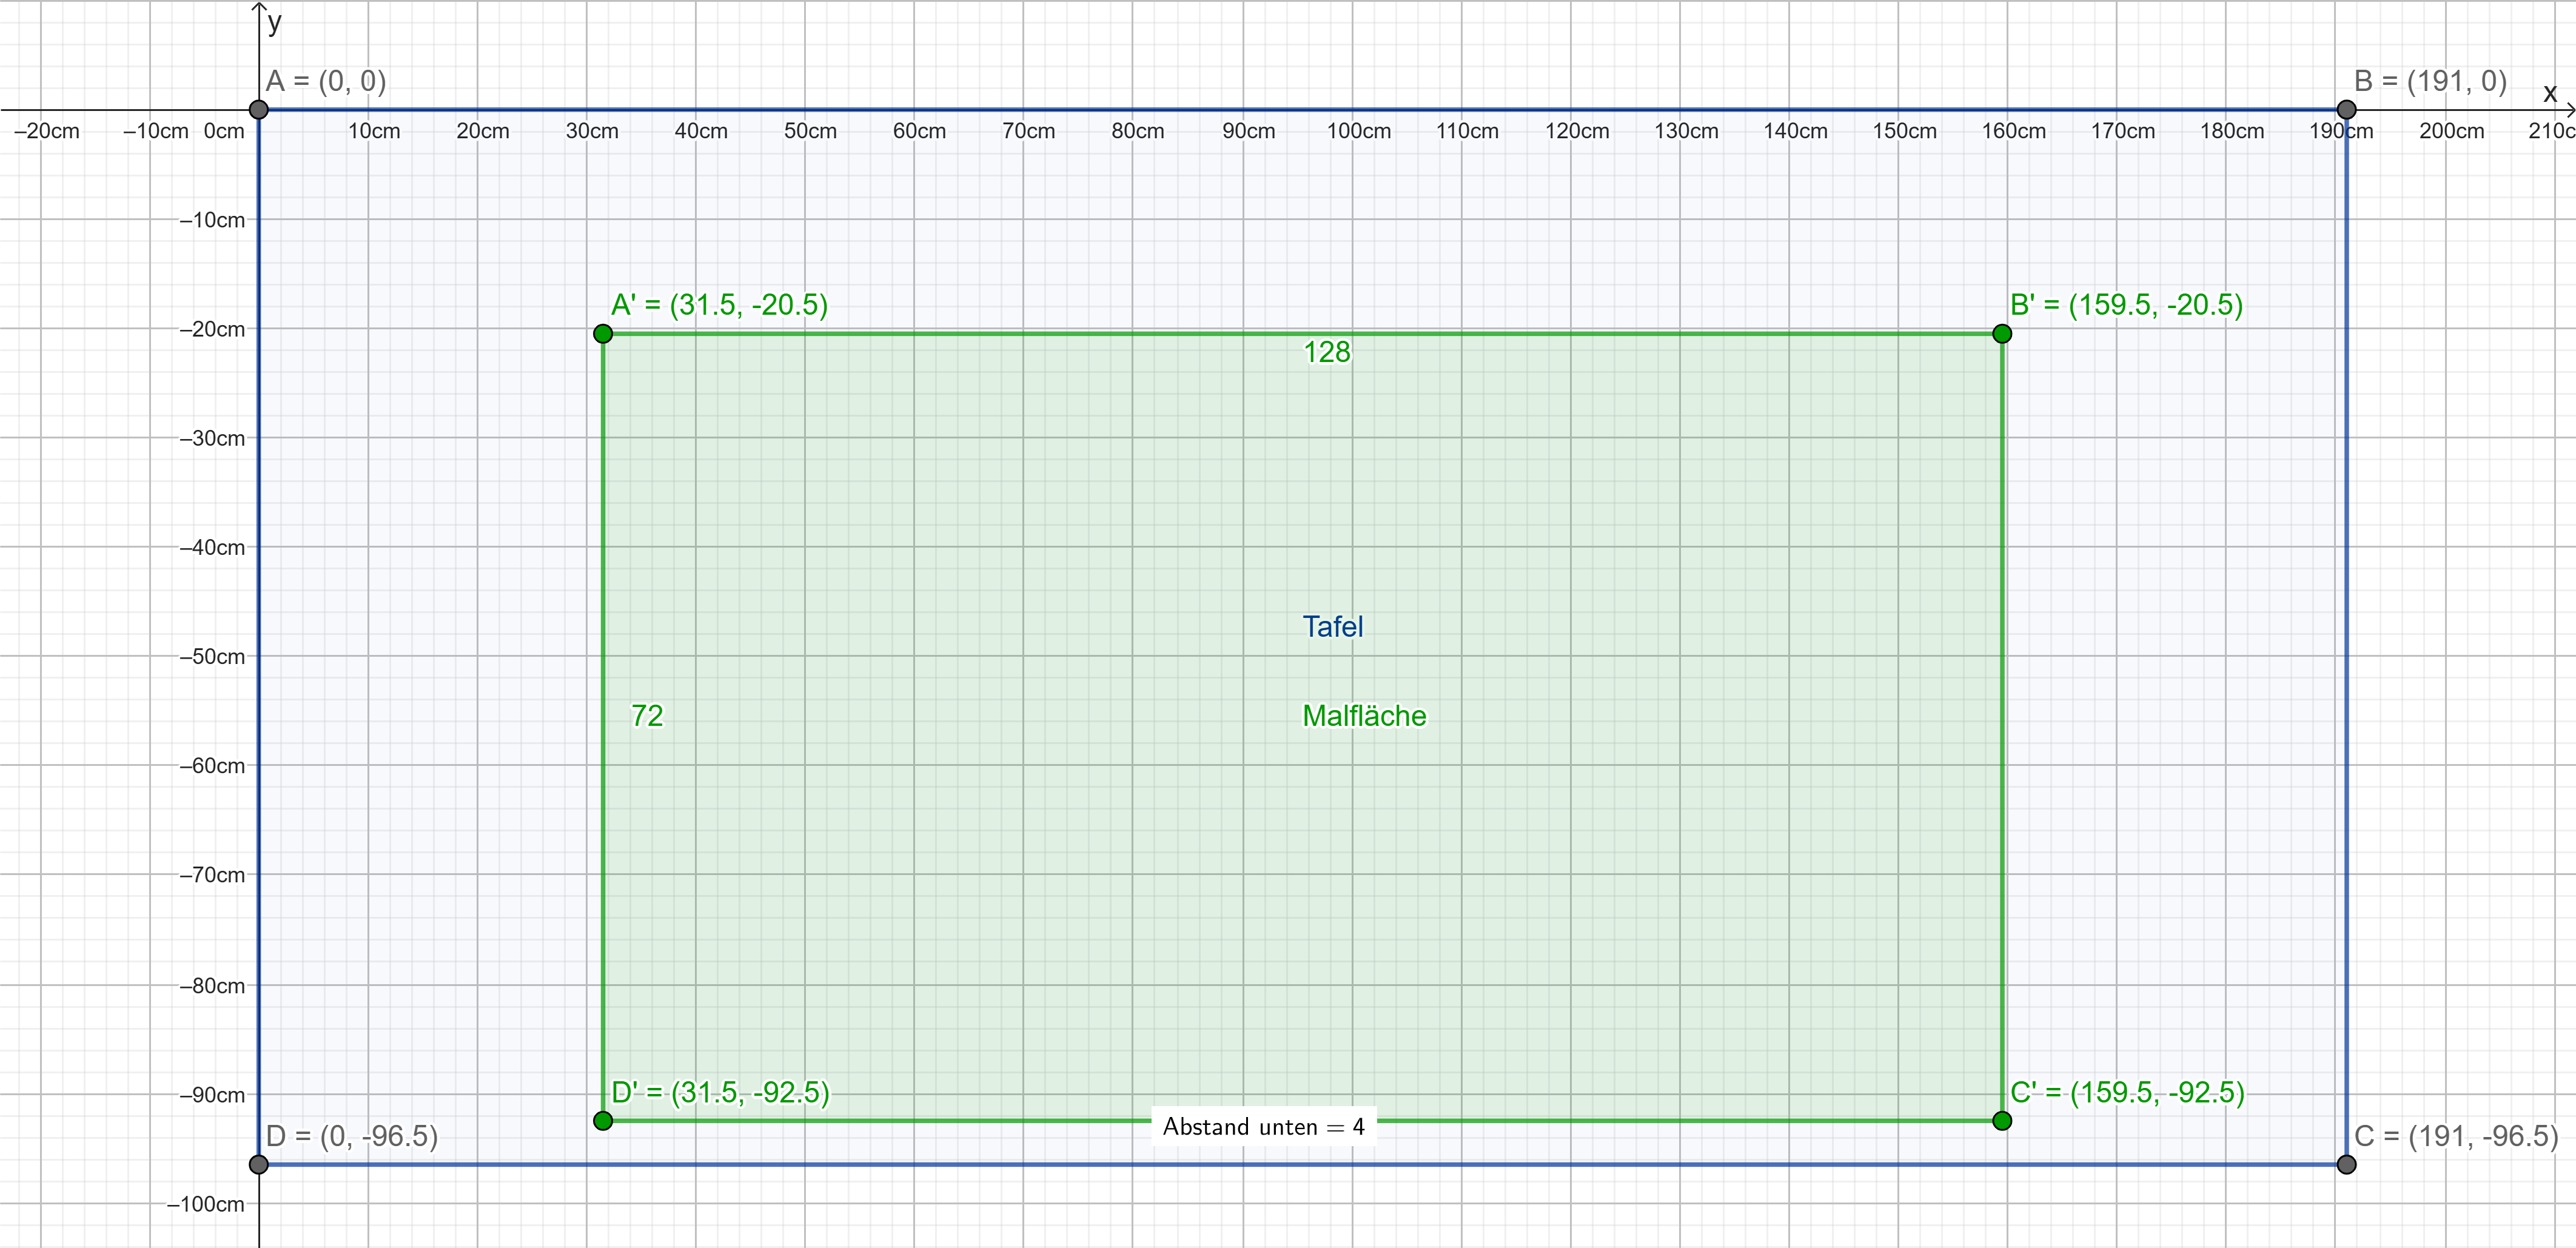
\includegraphics[width=\linewidth]{images/Tafelabmessungen.png}
\caption{Initiale Abmesssungen des benutzten Whiteboards}
\label{fig:abmessungen}
\end{figure}

Mit dem Einstellen einer gewünschten abzuarbeitenden Winkelsequenz beschäftigt sich der Reiter \glqq{}Angles-Config\grqq{}. Hier habe ich drei verschiedene Optionen implementiert: 

\begin{itemize}
\item Eine vordefinierte Winkelsequenz \glqq{}pre-build angles 1\grqq{}. Dieses Tupel von Winkelsequenzen und den dazugehörigen Zeiten sind im Code vordefiniert und stellen eine Boundingbox der Zeichenfläche dar (bei 8mm Spulendurchmesser und der initialen Zeichenfläche!) 
\item Wie oben, nur mit \glqq{}pre-build angles 2\grqq{} wird ein Dreieck gezeichnet (Hier wurde auch wieder mit einem Spulendurchmesser von 8mm gearbeitet, andere Durchmesser skalieren das Dreieck). 
\item Durch die letzte Option \glqq{}fileContent angles\grqq{} lassen sich auch nach Abb. \ref{fig:dateiformat} eigens definierte Winkelsequenzen innerhalb einer .txt Datei einlesen. Dazu wird intern mit einem von mir geschriebenen Parser der Inhalt der Datei in ein für JavaScript lesbares Tupel von 3-Tupeln (Zeit, Winkel MotorLinks, Winkel MotorRechts) übersetzt.  
\end{itemize}

Unter dieser Auswahl wird dem Benutzer die erste sowie letzte Zeile und die gesamte Anzahl an Winkelsequenzen der ausgewählten Datei angezeigt.

\begin{table}[H]
\caption{Funktionen aller HTML-Elemente der GUI; Von oben nach unten aufgelistet}
\centering
\begin{tabular}{p{2cm}|c|p{4cm}}
Name & Art & Funktion \\
\hline
Start & Button & Startet die Simulation \\
Pause/Resume & Button & Pausiert/Startet die Simulation \\
Reset & Button & Setzt die Simulation zurück \\
Versteck Seile\&Stift & Checkbox & Schaltet Ansicht des Vordergrunds an/aus \\
Versteck Koordinatensystem & Checkbox & Schaltet Ansicht des Koordinatensystems an/aus \\
Stop on errors & Checkbox & Entscheidet, ob Simulation bei Fehler stoppen/weiterlaufen soll \\
Diameter Coil & Slider & Eingabe des verwendeten Spulendurchmessers \\
Canvaswidth & Input & Eingabe Breite des Canvas \\
Canvasheigth & Input & Eingabe Höhe des Canvas \\
Drawwidth & Input & Eingabe Breite der Zeichenfläche \\
Drawheight & Input & Eingabe Höhe der Zeichenfläche \\
Start x & Input & Eingabe x-Koordinate Startpunkt \\
Start y & Input & Eingabe y-Koordinate Startpunkt \\
Use pre-build angles 1 & Radiobutton & Benutzt Winkelsequenzen, die eine Boundingbox ergeben \\
Use pre-build angles21 & Radiobutton & Benutzt Winkelsequenzen, die ein Dreieck ergeben \\
Use fileContent angles & Radiobutton & Benutzt eigens definierte Winkelsequenzen einer hochgeladenen Datei
\end{tabular}
\label{tab:gui_funcs}
\end{table}